\section{Approach}
\label{sec:approach}
\begin{figure}[t]
\centering
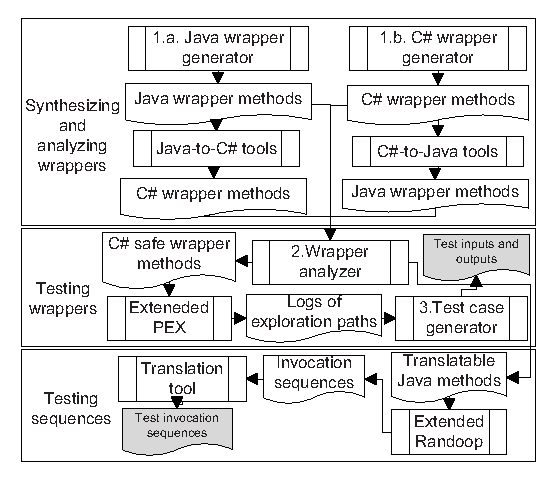
\includegraphics[scale=0.9,clip]{figure/approach.eps}\vspace*{-3ex}
 \caption{Overview of TeMAPI}\vspace*{-4ex}
 \label{fig:approach}
\end{figure}

As shown in Figure~\ref{fig:approach}, given a translation tool between Java and C\#, TeMAPI generates various test cases to reveal behavioral differences of API mapping relations defined by the tool.


%-------------------------------------------------------------------
\subsection{Synthesizing and Analyzing Wrappers}
\label{sec:approach:wrapper}
Given a translation tool, TeMAPI first extracts its API mapping relations. To deal with different formats of translation tools as described in Section~\ref{sec:introduction}, TeMAPI does not extract API mapping relations directly from translation tools, but analyzes translated code for such relations. As shown in Figure~\ref{fig:approach}, TeMAPI has a Java wrapper generater for Java-to-C\# tools and a C\# wrapper generater for C\#-to-Java tools. For static fields and static methods, the two wrapper generater of TeMAPI uses the following rules to synthesize wrapper methods. In the below synthesized code, ``\CodeIn{|f.name|}'' denotes the name of a field \CodeIn{f}; ``\CodeIn{|m.name|}'' denotes the name of a method \CodeIn{m}; and ``\CodeIn{|no|}'' denotes the number of synthesized wrapper method.

\textbf{Static fields.} Given a public static field \CodeIn{f} of a class \CodeIn{C} whose type is \CodeIn{T}, TeMAPI synthesizes a getter as follows:

\begin{CodeOut}\vspace*{-1.5ex}
\begin{alltt}
 public T testGet|f.name||no|sfg()\{ return C.f; \}
\end{alltt}
\end{CodeOut}\vspace*{-1.5ex}

If \CodeIn{f} is not a constant, TeMAPI synthesizes a setter as follows:

\begin{CodeOut}\vspace*{-1.5ex}
\begin{alltt}
 public void testSet|f.name||no|sfs(T v)\{ C.f = v; \}
\end{alltt}
\end{CodeOut}\vspace*{-1.5ex}

\textbf{Static methods.} Given a public static method \CodeIn{m(T1\ m1,\ldots,Tn\ mn)} of a class \CodeIn{C} whose return type is \CodeIn{Tm}, TeMAPI synthesizes a wrapper method as follows:

\begin{CodeOut}\vspace*{-1.5ex}
\begin{alltt}
 public Tm test|m.name||no|sm(T1\ m1,\ldots, Tn\ mn)\{
   return C.m(m1,\ldots, mn); \}
\end{alltt}
\end{CodeOut}\vspace*{-1.5ex}

When TeMAPI synthesizes wrapper methods for non-static fields or methods, it takes constructors into considerations:

\textbf{Non-static fields.} Given a public non-static field \CodeIn{f} of a class \CodeIn{C} whose type is \CodeIn{T}, TeMAPI synthesizes a getter using each constructor \CodeIn{C(T1\ c1,\ldots, Tn\ cn)} of \CodeIn{C} as follows:

\begin{CodeOut}\vspace*{-1.5ex}
\begin{alltt}
 public T testGet|f.name||no|nfg(T1\ c1,\ldots, Tn\ cn)\{
    C obj = new C(c1,\ldots, cn);
    return obj.f; \}
\end{alltt}
\end{CodeOut}\vspace*{-1.5ex}

If \CodeIn{f} is not a constant, TeMAPI synthesizes a setter as follows:

\begin{CodeOut}\vspace*{-1.5ex}
\begin{alltt}
 public void testSet|f.name||no|nfs(T v, T1\ c1,\ldots, Tn\ cn)\{
   C obj = new C(c1,\ldots, cn);
   obj.f = v; \}
\end{alltt}
\end{CodeOut}\vspace*{-1.5ex}

\textbf{Non-static methods.} Given a public non-static method \CodeIn{m(T1\ m1,\ldots,Tn\ mn)} of a class \CodeIn{C} whose return type is \CodeIn{Tm}, TeMAPI synthesizes a wrapper method using each constructor \CodeIn{C(Tv\ cv,\ldots, Tt\ ct)} of \CodeIn{C} as follows:

\begin{CodeOut}\vspace*{-1.5ex}
\begin{alltt}
 public Tm test|m.name||no|nm(T1\ m1,\ldots, Tn\ mn,
                            Tv cv, \ldots, Tt ct)\{
   C obj = new C(cv,\ldots, ct);
   return obj.m(m1,\ldots, mn); \}
\end{alltt}
\end{CodeOut}\vspace*{-1.5ex}


TeMAPI puts all synthesized wrapper methods for one API class $C$ to one synthesized class. When synthesizing, TeMAPI ignores generic methods, and when synthesizing for C\# API classes, it ignores \CodeIn{unsafe} methods, \CodeIn{delegate} methods, and methods whose parameters are marked as \CodeIn{out} or \CodeIn{ref} besides generic methods. Java does not have corresponding keywords, so existing translation tools typically do not translate the preceding methods. After wrappers are synthesized, we using the translation tool under analysis to translate them to the other language.

After synthesized code is translated, TeMAPI parses translated code and filters out wrapper methods with compilation errors. We use \emph{safe wrappers} to refer to the remaining wrapper methods. To identify wrapper methods with compilation errors, TeMAPI extends Visual Studio and Eclipse's Java compiler for C\# and Java code, respectively. Comparing source code of safe wrappers with source code of synthesized wrappers, TeMAPI extracts one-to-one mapping relations of API classes for the tool under analysis. For example, by comparing the first statements of the \CodeIn{testskip24nm} method in Java and in C\# as shown in Section~\ref{sec:example}, TeMAPI extracts the mapping relation between the \CodeIn{ByteArrayInputStream} class in Java and the \CodeIn{MemoryStream} class in C\#. Besides, TeMAPI also extracts translatable API methods for the tool under analysis. In the preceding example, TeMAPI adds \CodeIn{BufferedInput- Stream(InputStream)} constructor and the \CodeIn{skip(long)} method in Java to translatable API methods of JLCA since the wrapper method is translated from Java to C\# without complication errors.


\subsection{Testing Wrappers}
\label{sec:approach:single}
Wrappers are beneficial to detect behavioral differences for two factors. (1) wrapper methods expose all the inputs of its wrapped methods and constructors, so it is feasible to change values of inputs to exercise their paths; (2) each wrapper method has one constructor and one method at most, so it is easy to locate which method has behavioral differences. Due to the two factors, TeMAPI then extends Pex~\cite{tillmann2008pex} to generate test cases for safe wrapper methods for each API class in C\#. Basically, Pex repeatedly executes a method under test, so that it explores all feasible paths of the method. For each safe wrapper method, TeMAPI leverages Pex to explore its paths and internal paths of its called API methods. When exploring, TeMAPI records the inputs and the corresponding output of each unique feasible path to generate one test case. As each test case is generated from one unique path, each test case reflects one unique behavior. When generating test cases, TeMAPI refers to extracted mapping relations of API classes to translate C\# values into Java values. Vales of some primitive types can cause compilation errors, so TeMAPI replaces them with corresponding method invocations. For example, the \CodeIn{long m0 = 2147483648} statement causes a compilation error with a message: ``The literal 2147483648 of type int is out of range''. In Section~\ref{sec:example}, TeMAPI uses a method invocation to replace the statement in the \CodeIn{testskip24nm} test case. For objects, TeMAPI refers to extracts mapping relations of API classes to translate them. To check equivalence of outputs, TeMAPI checks whether their values are equal for primitive types and arrays, and checks whether each mapped fields are equal for objects. For example, TeMAPI records that given an empty object, the \CodeIn{testappend175nm} wrapper method in C\# returns a \CodeIn{StringBuilder} object whose \CodeIn{Capacity} field is 16 and \CodeIn{Length} field is 13, so TeMAPI generates a test case for the corresponding Java wrapper method as follows:

\begin{CodeOut}\vspace*{-1ex}
\begin{alltt}
public void testappend175nm122()\{
  Test_java_lang_StringBuffer obj =
      new Test_java_lang_StringBuffer();
  Object m0 = new Object();
  StringBuffer out = obj.testappend175nm(m0);
  Assert.assertEquals(16, out.capacity());	
  Assert.assertEquals(13, out.length());\}
\end{alltt}
\end{CodeOut}\vspace*{-2ex}

This test case fails, since here the \CodeIn{capacity()} method returns 34 and the \CodeIn{length()} method returns 24. Thus, TeMAPI detects two behavioral differences between the \CodeIn{java.lang.StringBuffer} class in Java and the \CodeIn{System.Text.StringBuilder} class in C\#.


We notice that when Pex explores a path with some specific inputs, the method under exploration throws exceptions.
For example, during exploring the \CodeIn{testvalueOf61sm} wrapper method in C\#, TeMAPI records that given a \CodeIn{null} input, the method throws \CodeIn{NullReferenceException}, so it generates a test case to ensure the corresponding Java wrapper method also throws a mapped exception. To generate the test case, TeMAPI first finds the corresponding exceptions in Java by analyzing translated wrapper methods with synthesized ones. In this example, TeMAPI finds that the \CodeIn{NullReferenceException} class in C\# is mapped to the \CodeIn{Null- PointerException} class in Java with respect to the API mapping relations of Java2CSharp, so it generates a Java test case as follows:

\begin{CodeOut}\vspace*{-1ex}
\begin{alltt}
 public void testvalueOf61sm3()\{
   try\{
     Test_java_lang_String obj =
           new Test_java_lang_String();
     java.lang.Object m0 = null;
     obj.testvalueOf61sm(m0);
   \}catch(java.lang.NullPointerException e)\{
     Assert.assertTrue(true);
     return;
   \}
   Assert.assertTrue(false); \}
\end{alltt}
\end{CodeOut}\vspace*{-1ex}

This test case gets failed since the \CodeIn{testvalueOf61sm} method in Java does not throw any exceptions given a null input.
From this failing test case, TeMAPI detects the behavioral difference between the \CodeIn{java.lang.String.valueOf(Object)} method in Java and the \CodeIn{System.Object.ToString()} method in C\#, since the preceding two wrapper methods are for the two API methods only.

%-----------------------------------------------------------
\subsection{Testing Invocation Sequences}
\label{sec:approach:sequence}
\begin{table}[t]
\centering
\begin{SmallOut}
\begin {tabular} {|c|l|c|c|c|c|c|c|}
 \hline
\textbf{Name}& \textbf{Version}& \textbf{Provider} &\textbf{Description}\\
\hline
Java2CSharp  &  1.3.4 & IBM (ILOG) & Java to C\# \\
\hline
JLCA         &  3.0   & Microsoft  & Java to C\# \\
\hline
sharpen      &  1.4.6 & db4o       & Java to C\# \\
\hline
Net2Java     &  1.0   & NetBean    &  C\# to Java\\
\hline
converter    &  1.6   & Tangible   &  C\# to Java\\
\hline
\end{tabular}\vspace*{-2ex}
\Caption{Subject tools} \label{table:subjects}
\end{SmallOut}\vspace*{-4ex}
\end{table}
Despite of its benefits to detect behavioral differences, a wrapper method is not appropriate to be used to test invocation sequences since it has fixed invocation sequences (\emph{e.g.}, a constructor first and then the public method). As a result, TeMAPI extends Randoop~\cite{pacheco2007feedback} to generate invocations sequences for all translatable API methods of the tool under analysis. Randoop randomly generates test cases based on already generated test cases in a feedback-directed manner, and it has both a Java version and a C\# version. When it generates test cases, TeMAPI limits its search scope within translatable API methods only. Generated test cases by Randoop have \CodeIn{assert} statements. TeMAPI runs generated test cases, and removes all failing test cases. We then use translation tools under analysis to translate remaining test cases to the other language. If translated code has the same behaviors, translated test cases should also get passed. If not, TeMAPI detects behavioral differences. Thus, TeMAPI does not need to generate assertion statements as it does to test wrappers. Section~\ref{sec:evaluation:sequence} shows such detected behavioral differences that are related to invocation sequences (\emph{e.g.}, the \CodeIn{test87} test cases).




